\documentclass[11pt,xcolor={dvipsnames},hyperref={pdftex,pdfpagemode=UseNone,hidelinks,pdfdisplaydoctitle=true},usepdftitle=false]{beamer}
\usepackage{presentation}

% Enter presentation title to populate PDF metadata:
\hypersetup{pdftitle={Minimalist LaTeX Template for Academic Presentations}}

% Enter path to PDF file with figures:
\newcommand{\pdf}{figures.pdf}

\begin{document}

% Enter title:
\title{Risk Models From Tree-Structured MRFs Following Multivariate Poisson Distributions}


\information
%
% Enter URL to research paper (can be commented out):
% [https://arxiv.org/pdf/2412.00607]
%
% Enter authors:
{
\Large Alexandre Dubeau\\
% \vspace{-1cm}
\smallskip \large Joint work with H. Cossette, B. Côté, and E. Marceau\\
\normalsize École d'actuariat, Université Laval}
%
% Enter location and date (can be commented out):
{Statistical Society of Canada Conference-- May 26 2025}

\frame{\titlepage}

\section{Introduction}
% \begin{frame}{Two Major Insurance Systems}
% \begin{minipage}[t]{0.45\textwidth}
% {\large Traditional Insurance}:
% \begin{itemize}
%     \item Centralized risk-sharing mechanism;
%     \item Insurer = intermediary;
%     \item Standardized contracts $\Rightarrow$ portfolio expansion.
%     % \item  Focus on predictability and accessibility
% \end{itemize}
% \end{minipage}
% \hfill
% \begin{minipage}[t]{0.45\textwidth}
% {\large Decentralized Insurance}\\
% \citep{feng2024unified}:
% \begin{itemize}
%     \item Removal of a central intermediary;
%     \item Reform of mutualization principles;
%     \item Use of modern technologies.
% \end{itemize}
% \end{minipage}
% \pause

% \vspace{5pt}

% {\large Common point: }
% \begin{itemize}
%     \item Based on risk pooling;
%     \item One of the objectives: \\
%     $\downarrow$ individual contributions through \al{risk sharing}.
% \end{itemize}
% \end{frame}
\begin{frame}{Dependent Risks in insurance}
\begin{itemize}
    \item Insurance portfolios often contain multiple risks affected by shared causes (e.g., floods, wildfires, cyber attacks).
    
    \item These shared causes induce dependence in claim occurrences.
    
    \item Accurately modeling this dependence is critical for:
    \begin{itemize}
        \item Portfolio-level risk assessment;
        \item Fair capital allocation among participants;
        \item Regulatory solvency metrics.
    \end{itemize}
    
    \item We aim to build flexible and tractable risk models for \al{dependent count data}, with actuarial relevance.
\end{itemize}
\end{frame}

\begin{frame}[label=toc]{Overview}
    \setlength{\leftskip}{5cm}%
    \tableofcontents[subsectionstyle=hide]
\end{frame}

\section{Individual Risk Models}
\begin{frame}{Individual Risk Model - Classical Framework}
Definition: 
\begin{itemize}
    \item Portfolio of $n$ participants $\boldsymbol{X} = (X_v)_{v=1}^{n}$.
    \item Each has a non-negative monetary loss $X_v, v \in [n] = \{1,2, \dots, n\}$.
    \item $\mu_v = \mathbb{E}[X_v] < \infty$, $\sigma_v^2 = \mathrm{Var}(X_v) < \infty$.
    \item Aggregate portfolio loss $S_n$:  
    \begin{equation*}
    S_n = X_1 + X_2 + \cdots + X_n.
    \end{equation*}
\end{itemize}
\vfill

\pause

Assumptions about the random variables $X_i$: 
\begin{itemize}
    \item identically distributed (homogeneous portfolio);
    \item independent. 
\end{itemize}
\end{frame}

\section{Compound Poisson Distribution individual risk models}
\begin{frame}
\frametitle{Relaxing the Classical Framework assumptions}
\begin{itemize}
    \item Portfolio of $n$ \al{heterogeneous} risks: $\boldsymbol{X} = (X_v)_{v=1}^{n}$.
    % with $X_v = \sum_{i=1}^{N_v} B_{v,i}$.

    \vfill

    \item Each risk $X_v$ in $\boldsymbol{X}$ follows a compound Poisson distribution: 
        \begin{equation*}
        X_v = \sum_{j=1}^{N_v} B_{v,j},
        \end{equation*}
        with $N_v \sim \text{Poisson}(\lambda_v)$ and $ \{B_{v,j}\}_{j \ge 1}$ are i.i.d. claim sizes for each $v \in [n]$.
        \pause

        \vfill

    \item We wish to introduce \al{dependence} in the portfolio through frequency distributions.
\end{itemize}

\end{frame}

%% Mentionner a voix haute sera mieux je pense. 
% \begin{frame}
% \frametitle{Multivariate Poisson Modeling with Poisson Marginals}
% \begin{itemize}
%         \item Copula-based methods:
%         \begin{itemize}
%             \item[+] Allow \alg[1-2]{separate modeling of marginals and dependence}
%             \item Often avoided in discrete contexts due to theoretical and computational challenges\\
%             \citep{genest2007primer, henn2022limitations}
%         \end{itemize}
        
%         \vfill
%         \pause
%         \item Common-Shock Models (MPCS):
%         \begin{itemize}
%         \item[$\rightarrow$] One shock event can trigger claims across multiple risks
%         \item[+] Provide \alg[2]{clear interpretation of dependence} mechanisms
%             % \item 
%             \item Parameter count grows exponentially with dimension
%             \item Becomes computationally intractable for large portfolios\\
%             \tiny \citep{karlis2003algorithm, ccekyay2023computing}
%         \end{itemize}
%         \vfill 
%         \item[$\Rightarrow$]  \cite{cote2025tree}: a tractable, interpretable framework based on tree-structured Markov random fields with Poisson marginals.
% \end{itemize}
% \end{frame} 

\section{Tree-structured Markov Random Field with Poisson marginal}
\begin{frame}{Notation: Tree-Structured Graphs}
\begin{columns}
    \begin{column}{0.6\textwidth}
        % \textbf{Tree Definition:}
        \begin{itemize}
            \item A tree $\mathcal{T}=(\mathcal{V},\mathcal{E})$ is a graph where:
            \begin{itemize}
                \item $\mathcal{V}=\{1,\ldots,d\}$ is the set of vertices;
            \item $\mathcal{E} \subseteq \{\{u,v\} : u,v \in \mathcal{V}, u \neq v\}$ is the set of undirected edges;
            \item \al{No cycle} or loop exist.
            \end{itemize}
            % \pause
            \item $\mathrm{path}(u, v)$: set of edges connecting vertex $u$ to vertex $v$, $u,v \in \mathcal{V}$.
            % \pause
            \item We designate one vertex as the \al{root} $r$.
            \item For each vertex $v$:
            \begin{itemize}
                \item $\mathrm{pa}(v)$: parent of $v$;
                \item $\mathrm{ch}(v)$: set of children of $v$.
                \item $\mathrm{dsc}(v)$: set of descendants of $v$.
            \end{itemize}
        \end{itemize}
    \end{column}
    % \pause
    \begin{column}{0.4\textwidth}
    \onslide*<1>{\resizebox{0.8\textwidth}{!}{% \usepackage{mathrsfs}
% \begin{tikzpicture}[
%   grow cyclic, 
%   level distance=0.8cm, 
%   level 1/.style={sibling angle=120, nodes={fill=Violet!75, circle, draw, thick}},
%   level 2/.style={sibling angle=70, nodes={fill=Violet!45, circle, draw, thick}},
%   level 3/.style={sibling angle=55, nodes={fill=Violet!30, circle, draw, thick}},
%   level 4/.style={sibling angle=45, nodes={fill=Violet!10, circle, draw, thick}},
%   edge from parent/.style={draw, thick},
%   edge from parent path={(\tikzparentnode) -- (\tikzchildnode)},
%   scale = 0.6
% ]

% \node [circle, draw, fill=Violet, thick] {} % racine node
%   child {node {} % niveau 2
%     child {node {} % niveau 3
%       child {node {} % niveau 4
%         child {node {}} % niveau 5
%         child {node {}} % niveau 5
%       }
%       child {node {} % niveau 4
%         child {node {}} % niveau 5 
%         child {node {}} % niveau 5
%       }
%     }
%     child {node {} % niveau 3
%       child {node {} % niveau 4
%         child {node {}} % niveau 5
%         child {node {}}  % niveau 5
%       }
%       child {node {}  % niveau 4
%         child {node {}} % niveau 5
%         child {node {}} % niveau 5
%       }
%     }
%   }
%   child {node {} % niveau 2
%     child {node {} % niveau 3
%       child {node {} % niveau 4
%         % child {node {}} % niveau 5
%         % child {node {}} % niveau 5
%       }
%       child {node {} % niveau 4
%         % child {node {}} % niveau 5 
%         % child {node {}} % niveau 5
%       }
%     }
%     child {node {} % niveau 3
%       child {node {} % niveau 4
%         child {node {}} % niveau 5
%         child {node {}}  % niveau 5
%       }
%       child {node {}  % niveau 4
%         % child {node {}} % niveau 5
%         % child {node {}} % niveau 5
%       }
%     }
%   }
%   child {node {} % niveau 2
%     child {node {} % niveau 3
%       child {node {} % niveau 4
%         % child {node {}} % niveau 5
%         % child {node {}} % niveau 5
%       }
%       child {node {} % niveau 4
%         child {node {}} % niveau 5 
%         child {node {}} % niveau 5
%       }
%     }
%     child {node {} % niveau 3
%       child {node {} % niveau 4
%         child {node {}} % niveau 5
%         child {node {}}  % niveau 5
%       }
%       child {node {}  % niveau 4
%         % child {node {}} % niveau 5
%         % child {node {}} % niveau 5
%       }
%     }
%   };

% \end{tikzpicture}
\begin{tikzpicture}[
  grow cyclic, 
  level distance=0.8cm, 
  level 1/.style={sibling angle=120, nodes={circle, draw, thick}},
  level 2/.style={sibling angle=70, nodes={circle, draw, thick}},
  level 3/.style={sibling angle=55, nodes={circle, draw, thick}},
  level 4/.style={sibling angle=45, nodes={circle, draw, thick}},
  level 5/.style={sibling angle=15, nodes={draw =none, font = \footnotesize, transform shape}},
  edge from parent/.style={draw, thick},
  edge from parent path={(\tikzparentnode) -- (\tikzchildnode)},
  scale = 0.6
]

\node (1) [circle, draw, thick, fill = black] {} % racine node
  child {node {} % niveau 2
    child {node {} % niveau 3
      child {node {} % niveau 4
        child {node {}} % niveau 5
        child {node {}} % niveau 5
      }
      child {node {} % niveau 4
        % child {node {}} % niveau 5 
        % child {node {}} % niveau 5
      }
    }
    child {node {} % niveau 3
      child {node {} % niveau 4
        child {node {}} % niveau 5
        child {node {}}  % niveau 5
      }
      child {node {}  % niveau 4
        % child {node {}} % niveau 5
        % child {node {}} % niveau 5
      }
    }
  }
  child {node {} % niveau 2
    child {node {} % niveau 3
      child {node {} % niveau 4
        child {node {}} % niveau 5
        child {node {}} % niveau 5
      }
      child {node {} % niveau 4
        % child {node {}} % niveau 5 
        % child {node {}} % niveau 5
      }
    }
    child {node {} % niveau 3
      child {node {} % niveau 4
        child {node {}} % niveau 5
        child {node {}}  % niveau 5
      }
      child {node {}  % niveau 4
        % child {node {}} % niveau 5
        % child {node {}} % niveau 5
      }
    }
  }
  child {node {} % niveau 2
    child {node {} % niveau 3
      child {node {} % niveau 4
        % child {node {}} % niveau 5
        % child {node {}} % niveau 5
      }
      child {node {} % niveau 4
        child {node {}} % niveau 5 
        child {node {}} % niveau 5
      }
    }
    child {node {} % niveau 3
      child {node {} % niveau 4
        child {node {}
        } % niveau 5
        child {node {}}  % niveau 5
      }
      child {node {}  % niveau 4
        % child {node {}} % niveau 5
        % child {node {}} % niveau 5
      }
    }
  };
\end{tikzpicture}}
    
    \centering \hspace{-1cm} Tree $\mathcal{T}_{\bullet}$
    }
    \onslide*<2>{\resizebox{0.8\textwidth}{!}{\begin{tikzpicture}[
  grow cyclic, 
  level distance=0.8cm, 
  level 1/.style={sibling angle=120, nodes={circle, draw, thick}},
  level 2/.style={sibling angle=70, nodes={circle, draw, thick}},
  level 3/.style={sibling angle=55, nodes={circle, draw, thick}},
  level 4/.style={sibling angle=45, nodes={circle, draw, thick}},
  level 5/.style={sibling angle=15, nodes={draw =none, font = \footnotesize, transform shape}},
  edge from parent/.style={draw, thick},
  edge from parent path={(\tikzparentnode) -- (\tikzchildnode)},
  scale = 0.6
]

\node (1) [circle, draw, thick, fill = black] {} % racine node
  child {node (A) {} % niveau 2
    child {node {} % niveau 3
      child {node {} % niveau 4
        child {node {}} % niveau 5
        child {node {}} % niveau 5
      }
      child {node {} % niveau 4
        % child {node {}} % niveau 5 
        % child {node {}} % niveau 5
      }
    }
    child {node {} % niveau 3
      child {node {} % niveau 4
        child {node {}} % niveau 5
        child {node {}}  % niveau 5
      }
      child {node (C) {}  % niveau 4
        % child {node {}} % niveau 5
        % child {node {}} % niveau 5
      }
    }
  }
  child {node (B) {} % niveau 2
    child {node {} % niveau 3
      child {node {} % niveau 4
        child {node {}} % niveau 5
        child {node {}} % niveau 5
      }
      child {node {} % niveau 4
        % child {node {}} % niveau 5 
        % child {node {}} % niveau 5
      }
    }
    child {node {} % niveau 3
      child {node  {} % niveau 4
        child {node {}} % niveau 5
        child {node {}}  % niveau 5
      }
      child {node (D) {}  % niveau 4
        % child {node {}} % niveau 5
        % child {node {}} % niveau 5
      }
    }
  }
  child {node  {} % niveau 2
    child {node {} % niveau 3
      child {node {} % niveau 4
        % child {node {}} % niveau 5
        % child {node {}} % niveau 5
      }
      child {node {} % niveau 4
        child {node {}} % niveau 5 
        child {node {}} % niveau 5
      }
    }
    child {node {} % niveau 3
      child {node {} % niveau 4
        child {node {}
        } % niveau 5
        child {node {}}  % niveau 5
      }
      child {node {}  % niveau 4
        % child {node {}} % niveau 5
        % child {node {}} % niveau 5
      }
    }
  };
% Add an extra edge to create a cycle (making it not a tree)
\draw[red, thick, line width = 2pt] (B) to[] (C);

\end{tikzpicture}}
    
    \centering
    
    \hspace{-1cm} Not a tree
    }
    \end{column}
\end{columns}
\end{frame}
\begin{frame}
\frametitle{Tree-structured Markov Random Fields (MRFs)}
\begin{block}{Definition: Markov Random Field on a Tree}
    A vector of random variables $\boldsymbol{N}= (N_v, \, v \in \mathcal{V})$ defined on tree $\mathcal{T} = (\mathcal{V},\mathcal{E})$, is a MRF if it satisfies the 
    \al{global Markov property}:
\end{block}

\onslide<2->{
\begin{tikzpicture}[overlay, remember picture]
\node[anchor=west] at ([xshift=-6cm, yshift=-0.5cm]current page.center) (markov) {Two random variables are conditionally independent,};
\node[anchor=west] at ([xshift=-6cm, yshift=-1cm]current page.center) (markov2) {given the value of any random variable on the path between them.};
\draw[->, thick, >=stealth, line width = 1.5pt] ([xshift=-2cm, yshift=-3.3cm]current page.north)  to[out=220, in=180]([xshift=-4cm]markov.north)  node[] {};
\end{tikzpicture}
}

\vspace{2.5cm}
\onslide<3->{
\textbf{Key advantages:} Tree-structured MRFs enable efficient 
\begin{itemize}
    \item algorithms for computation (\cite{wainwright2003tree});
    \item structure learning \citep{bresler2020learning, nikolakakis2021predictive}.
\end{itemize}
}
\end{frame}

\begin{frame}{A Balanced Solution to Multivariate Poisson Modeling with Poisson Marginals}
Tree-structured MRFs with Poisson marginals \citep{cote2025tree} 
\begin{itemize}
        \item[+] \alg{Preserves Poisson marginals} while introducing dependence;
        \vfill
        \item[+] Parameter count grows \alg{linearly with dimension} 
        (not exponentially)
        \vfill
        \item[+] \alg{Computationally tractable} for large portfolios
        \vfill
        \item[+] \alg{Provides clear interpretation} of dependence structure
        \vfill
        \item[$-$] Allows for \alr{only one mean parameter} $\lambda$ for all $N_v, v \in \mathcal{V}$ 
\end{itemize}
\end{frame}
\begin{frame}{Flexible Tree-structured MRFs with Poisson marginals}
    % Let
    \begin{itemize}
            \item Tree $\mathcal{T} = (\mathcal{V}, \mathcal{E})$;
            \item Parameters: means $\boldsymbol{\lambda} = (\lambda_v)_{v \in \mathcal{V}}$ and dependencies $\boldsymbol{\alpha} = (\alpha_e)_{e \in \mathcal{E}}$;
            \item Constraint: $\alphav{v} \in [0, \min(\sqrt{{\lambda_{v}}/{\lambda_{\pa{v}}}}, \sqrt{{\lambda_{\pa{v}}}/{\lambda_{v}}})]$;
         \item  "$\circ$" is the binomial thinning operator: $(\alpha\circ N) \sim$ Binomial$(N,\alpha)$.
    \end{itemize}
    \pause
\begin{theorem}
For a given root $r \in \mathcal{V}$, let $\boldsymbol{N}$ have the following recursive construction:
        \begin{equation*}
        N_v = 
        \begin{cases}
        L_r, & \text{if } v = r, \\ 
        \alphav{v} \sqrt{\dfrac{\lambda_v}{\lambda_{\pa{v}}}} \circ N_{\pa{v}} + L_v, & \text{otherwise},
        \end{cases}
        \vspace{-0.1cm}
        \end{equation*}
        where $\boldsymbol{L} = (L_v)_{v\in\mathcal{V}}$ are independent Poisson variables with $\lambda_{L_v} = \lambda_v- \alphav{v}\sqrt{\lambda_{\pa{v}}\lambda_v}$.
        
        Then $\boldsymbol{N} \sim \text{MPMRF}(\boldsymbol{\lambda}, \boldsymbol{\alpha}, \mathcal{T})$ with marginals $N_v \sim \text{Poisson}(\lambda_v)$.
\end{theorem}
    

\end{frame}


\begin{frame}
\frametitle{Understanding the stochastic construction}
Let $\boldsymbol{N} = (N_1,\dots, N_7) \sim \text{MPMRF}(\boldsymbol{\lambda}, \boldsymbol{\alpha}, \mathcal{T})$ as in Theorem 1.    
        \begin{example}
            % Consider $\boldsymbol{N} = (N_1,\dots, N_7)$  defined on the tree $\mathcal{T}$ depicted below. 
        \begin{figure}[H] 
            \centering
            \begin{minipage}[b]{0.30\textwidth}
            \centering
            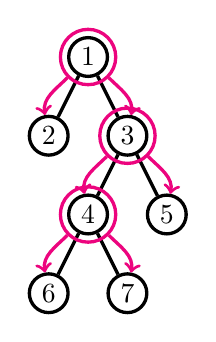
\begin{tikzpicture}[xscale = 1, yscale = 1, very thick]
                \tikzstyle{vertex}=[circle, draw = black,fill=white,minimum size=14pt,inner sep=0pt]
                
                \foreach \name/\x/\y in {1/0/3, 2/-0.5/2, 3/0.5/2, 4/0/1, 5/1/1, 6/-0.5/0, 7/0.5/0}
                \node[vertex] (G-\name) at (\x,\y) {\name};
                
                \foreach \from/\to in {1/2, 1/3, 3/4, 3/5, 4/6, 4/7}
                \draw (G-\from) -- (G-\to);
    
        \node<2->[circle, draw = RubineRed, very thick, minimum size = 20pt, fill = none](emph1) at (0,3){};
        
        \draw<3->[RubineRed, very thick, ->] (emph1) to [out = 225, in=100] (G-2);
        
        \draw<4->[RubineRed, very thick, ->] (emph1) to [out = 315, in=80] (G-3);
        
        \node<5->[circle, draw = RubineRed, very thick, minimum size = 20pt, fill = none](emph3) at (0.5,2){};
    
         \draw<6->[RubineRed, very thick, ->] (emph3) to [out = 225, in=100] (G-4);
    
        \draw<7->[RubineRed, very thick, ->] (emph3) to [out = 315, in=80] (G-5);
    
        \node<7->[circle, draw = RubineRed, very thick, minimum size = 20pt, fill = none](emph4) at (0,1){};
    
      \draw<7->[RubineRed, very thick, ->] (emph4) to [out = 225, in=100] (G-6);
    
        \draw<7->[RubineRed, very thick, ->] (emph4) to [out = 315, in=80] (G-7);
       
            \end{tikzpicture}
            \end{minipage}
            \hfill
            \begin{minipage}[b]{0.69 \textwidth}
                Stochastic construction, root = 1
                \medskip\\
                \onslide<2->{$N_1 = L_1,\phantom{+\;\alpha_{(v,2)}\circ N_1}\quad L_1\sim$ Poisson$(\lambda_{L_1})$}\\
                \onslide<3->{$N_2 = \alpha_{(1,2)}\circ N_1 + L_2,\quad L_2\sim$ Poisson$(\lambda_{L_2})$}\\
                \onslide<4->{$N_3 = \alpha_{(1,3)}\circ N_1 + L_3,\quad L_3\sim$ Poisson$(\lambda_{L_3})$}\\
                \onslide<6->{$N_4 = \alpha_{(3,4)}\circ N_3 + L_4,\quad L_4\sim$ Poisson$(\lambda_{L_4})$}\\
                % \onslide<7->{$N_5 = \alpha_{(3,5)}\circ N_3 + L_5,\quad L_5\sim$ Poisson$(\lambda_{L_5})$}\\
                \onslide<7->{$\vdots$}\\
                % \onslide<9->{$N_6 = \alpha_{(4,6)}\circ N_4 + L_6,\quad L_6\sim$ Poisson$(\lambda_{L_6})$}\\
                \onslide<7->{$N_7 = \alpha_{(4,7)}\circ N_4 + L_7,\quad L_7\sim$ Poisson$(\lambda_{L_7})$}
            \end{minipage}
        \end{figure}
     \vspace{-0.3cm}
        
     where 
     \vspace{-0.3cm}
     \begin{itemize}
         \item  "$\circ$" is the binomial thinning operator: $(\alpha\circ N) \sim$ Binomial$(N,\alpha)$;
         \item $\lambda_{L_v} = \lambda_v - \alphav{v}\sqrt{\lambda_{\pa{v}}\lambda_v}, \; v \in \mathcal{V}$.
     \end{itemize}         

        \end{example}
\end{frame}

% \begin{frame}{An efficient subfamily of the multivariate Poisson distribution based on common shocks}
% Let \begin{itemize}
%     \item $\boldsymbol{N} \sim \text{MPMRF}(\boldsymbol{\lambda}, \boldsymbol{\alpha}, \mathcal{T})$ as in Theorem 1.
%     \item $\Theta_v$ be the set of all connected subsets of the tree $\mathcal{T}$ to $v$
% \end{itemize}
% \begin{theorem}
% $\boldsymbol{N}$ admits a common-shock representation:
%     \begin{equation*}
%     N_v = \sum_{\mathcal{W} \in \Theta_v} Y_{\mathcal{W}}, \quad v \in \mathcal{V},
%     \end{equation*}
%     % where $\mathcal{W}$ ranges over all , 
%     where $Y_{\mathcal{W}} \sim \text{Poisson}(\gamma_{\mathcal{W}})$ are independent and
%     {\color{DarkGray} 
%     \begin{equation*}
%      \gamma_{\mathcal{W}} = \left( \prod_{w\in \mathcal{W}} \lambda_w \right)\left(\prod_{(u,w)\in\mathcal{E}_{\mathcal{W}}} \frac{\alpha_{(u,w)}}{\sqrt{\lambda_u\lambda_v}}\right)\left(\prod_{(i,j)\in\mathcal{E}^{\dagger}_{\mathcal{W}}} \left(1-\alpha_{(i,j)}\sqrt{\frac{\lambda_j}{\lambda_i}}\right)\right), 
%      % \quad \mathcal{W}\in \bigcup_{v\in\mathcal{V}}\Theta_v,
%      \end{equation*}
%      with $\mathcal{E}_{\mathcal{W}} = \{(i,j)\in\mathcal{E} : i,j\in \mathcal{W}\}$ and $\mathcal{E}_{\mathcal{W}}^{\dagger} = \{(i,j)\in\mathcal{E} : i\in \mathcal{W}, j\not\in \mathcal{W}\}$.
%      }
% \end{theorem}
\begin{frame}{An Efficient Subfamily of Multivariate Poisson Based on Common Shocks}
\begin{theorem}
Let $\boldsymbol{N} \sim \text{MPMRF}(\boldsymbol{\lambda}, \boldsymbol{\alpha}, \mathcal{T})$. Then $\boldsymbol{N}$ admits a common-shock representation:
    \begin{equation*}
    N_v = \sum_{\mathcal{W} \in \Theta_v} Y_{\mathcal{W}}, \quad v \in \mathcal{V},
    \end{equation*}
    where:
    \begin{itemize}
        \item $\Theta_v$ is the set of all connected subsets of tree $\mathcal{T}$ containing vertex $v$;
        \item $Y_{\mathcal{W}} \sim \text{Poisson}(\gamma_{\mathcal{W}}), \mathcal{W} \in \Theta_v$ are independent random variables;
        \item $\gamma_{\mathcal{W}}$ are parameters derived from $\boldsymbol{\lambda}$ and $\boldsymbol{\alpha}$.
    \end{itemize}
\end{theorem}

\vspace{0.3cm}
\begin{itemize}
    \item Result: The MPMRF family ($\mathbb{MRMRF})$ is an \al{efficient subfamily} of the multivariate Poisson common shock family ($\mathbb{MPCS}$). 
    % \item \alg{Advantages}: Linear parameter growth ($2d-1$ vs $2^d$) while maintaining flexibility
    % \item \alg{Key insight}: Tree structure enables efficient representation of complex dependencies
\end{itemize}
\end{frame}
\begin{frame}{An Efficient Subfamily : An Example}
\begin{minipage}{0.69\textwidth}
    \begin{itemize}
    \item A $d=7$ multivariate distribution in $\mathbb{MPCS}$  requires $2^7 = 128$ parameters.
    \pause
    \vfill
    \item A MPMRF on $\mathcal{T}$ (in MPCS representation) requires $|\cup \Theta_v| + d = 46$ 
    % requires $f(v) = \prod_{u \in \mathrm{ch}(v)} \left(1 + f(u)\right) = 39$ 
    parameters.
    \pause
    \vfill
    \item The MPMRF stochastic representation requires $2d - 1 + d  = \al{20}$ \al{parameters}
    % \item MPMRF models are a subfamily of multivariate Poisson distributions with common shocks, with tree-structured shock subsets.
   
    % \item However:
    % \begin{itemize}
    %     \item Still requires up to $|\bigcup \Theta_v| = \mathcal{O}(2^d)$ shocks in general;
    %     \item Dependence and marginals become entangled in the $\gamma_{\mathcal{W}}$ parameters;
    %     \item Breaks the separability property of MPMRFs.
    % \end{itemize}
    
    % \item MPMRFs allow complex dependence with only $2d - 1$ parameters, while remaining computationally tractable.
\end{itemize}
\end{minipage}
\hfill
\begin{minipage}{0.30\textwidth}
\centering
\vfill
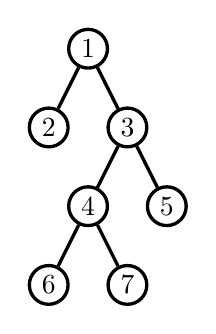
\begin{tikzpicture}[xscale = 1, yscale = 1, very thick]
    \tikzstyle{vertex}=[circle, draw = black,fill=white,minimum size=14pt,inner sep=0pt]
    
    \foreach \name/\x/\y in {1/0/3, 2/-0.5/2, 3/0.5/2, 4/0/1, 5/1/1, 6/-0.5/0, 7/0.5/0}
    \node[vertex] (G-\name) at (\x,\y) {\name};
    
    \foreach \from/\to in {1/2, 1/3, 3/4, 3/5, 4/6, 4/7}
    \draw (G-\from) -- (G-\to);
\end{tikzpicture}
% \vspace{1cm}

\hspace{-0.6cm} Tree $\mathcal{T}$
\vfill
\end{minipage}
\vfill
\pause
Conclusion : 
\begin{itemize}
    % \item     \vspace{1cm}
    \item \al{MPMRF scales as $\mathcal{O}(d)$} unlike the exponential cost of MPCS models.
    \item MPMRF retains \al{rich and tractable dependence} via tree structures.
    \item The recursive construction allows for \al{efficient computations}.
    % \item[$\Rightarrow$] 
\end{itemize}
\end{frame}
% \pause
% \vfill
% \begin{itemize}
    % \item MPMRF models are a subfamily of multivariate Poisson distributions with common shocks, with tree-structured shock subsets.
   
    % \item However:
    % \begin{itemize}
    %     \item Still requires up to $|\bigcup \Theta_v| = \mathcal{O}(2^d)$ shocks in general;
    %     \item Dependence and marginals become entangled in the $\gamma_{\mathcal{W}}$ parameters;
    %     \item Breaks the separability property of MPMRFs.
    % \end{itemize}
    
    % \item MPMRFs allow complex dependence with only $2d - 1$ parameters, while remaining computationally tractable.
% \end{itemize}
% \end{frame}
\section{Risk models with tree-structured MPMRF frequency distributions}
\begin{frame}{Risk model under the MPMRF framework}
Recall the framework: 
\begin{itemize}
    \item Portfolio of $n$ risks: $\boldsymbol{X} = (X_v)_{v=1}^{n}$ with $X_v = \sum_{j=1}^{N_v} B_{v,j}$.
    \vfill
    \item Dependence is introduced through the claim count vector $\boldsymbol{N}$:
    \begin{itemize}
        \item $\{B_{v,j}\}_{j \ge 1}$ i.i.d. for each $v$, independent of $\boldsymbol{N}$ and of $B_u, u \neq v$;
        \vfill    
        \item $\boldsymbol{N} \sim \text{MPMRF}(\boldsymbol{\lambda}, \boldsymbol{\alpha}, \mathcal{T}).$ 
    \end{itemize}
\end{itemize}

\begin{theorem}
The joint Laplace-Stieltjes transform (LST) of $\boldsymbol{X}$ can be expressed using the probability generating function of $\boldsymbol{N}$:
\begin{equation*}
\mathcal{L}_{\boldsymbol{X}}(\boldsymbol{t}) = \mathcal{P}_{\boldsymbol{N}}(\mathcal{L}_{B_1}(t_1), \dots, \mathcal{L}_{B_d}(t_d))
\end{equation*}    
    % \vfill
    % Objectives:
    % \begin{enumerate} 
    %     \item Develop efficient methods to evaluate its pmf/TLS without resorting to approximations  
    %     \item Evaluate the aggregate risk of the portfolio by studying the distribution of $S_n = \sum_{v \in \mathcal{V}} X_v$
    %     \item Assess the contribution of every component of the portfolio $\boldsymbol{X}$ to the aggregate claim amount
    % \end{enumerate}
\end{theorem}
% \al{Key result}: 
The tree structure allows for an efficient and exact computation of
% which enables:
\begin{itemize}
    \item the properties of $S_n$ through $\mathcal{P}_{S_n}(t) =  \mathcal{P}_{\boldsymbol{N}}(\mathcal{L}_{B_1}(t), \dots, \mathcal{L}_{B_d}(t))$;
    \item risk measures and the contributions of each risk.
\end{itemize}
\end{frame}

\begin{frame}{Numerical Illustrations Settings}
\begin{itemize}
    \item Portfolio of 31 risks;
    \item Poisson frequencies with $\lambda_v \sim  U(0.9,1.1)$ for all $v$;
    \item Geometric severities, $B_{v,i} \sim \text{Geom}(q_v),$ with $q_v \sim Unif(0,18, 0.22)$;
    \item Dependency parameter: $\alpha_e = 0.5$ for all edges.
\end{itemize}
% \resizebox{!}{0.8\textwidth}
% {\begin{tabular}{cccc}
% Structure A - Star

\begin{tikzpicture}[every node/.style={circle, draw, inner sep=2pt, minimum size=6mm}, scale = 0.35, transform shape]
    \tikzstyle{vertex}=[circle, draw = blue!60!white,fill=White,minimum size=10pt,inner sep=0pt, line width = 1.1pt]
    
    \foreach \label in {2,3,4,5,6,7,8,9}
    {
    \draw  (0,0) -- ({(\label-2)*12}:2cm);
    \node[vertex] (\label) at ({(\label-2)*12}:2cm) {\makebox[0.35cm][c]{\makebox[0.35cm][c]{}}};
    }
    \foreach \label in {10,11,12,13,14,15,16,17,18,19,20,21,22,23,24,25,26,27,28,29,30,31}
    {
    \draw  (0,0) -- ({(\label-2)*12}:2cm);
    \node[vertex] (\label) at ({(\label-2)*12}:2cm) {\makebox[0.35cm][c]{}};
    }
    \node[vertex] (base) at (0,0) {};
\end{tikzpicture} &

% Structure B - 5-nary tree
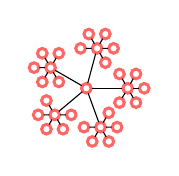
\begin{tikzpicture}[every node/.style={circle, draw, inner sep=2pt, minimum size=6mm}, scale = 0.35, transform shape]
    \tikzstyle{vertex}=[circle, draw = red!60!white,fill=White,minimum size=10pt,inner sep=0pt, line width = 1.1pt]
    
    \node[vertex] (base) at (0,0) {};
    
    \foreach \labelngle/\label in {75/2, 360/8, 290/14, 220/20, 150/26}{
        \node[vertex] (noeud\label) at (\labelngle:1.5cm) {\makebox[0.35cm][c]{}};
        \draw (base) -- (noeud\label);
    }
    
    \foreach \labelngle/\label in {360/4, 60/5, 120/6, 180/7, 300/3}{
        \node[vertex] (noeud\label) at ([shift={(\labelngle:0.6cm)}]noeud2) {\makebox[0.35cm][c]{}};
        \draw (noeud2) -- (noeud\label);
    }
    
    \foreach \labelngle/\label in {360/10, 60/11, 120/12, 240/13, 300/9}{
        \node[vertex] (noeud\label) at ([shift={(\labelngle:0.6cm)}]noeud8) {\makebox[0.35cm][c]{}};
        \draw (noeud8) -- (noeud\label);
    }
    
    \foreach \labelngle/\label in {60/15, 360/16, 300/17, 240/18, 180/19}{
        \node[vertex] (noeud\label) at ([shift={(\labelngle:0.6cm)}]noeud14) {\makebox[0.35cm][c]{}};
        \draw (noeud14) -- (noeud\label);
    }
    
    \foreach \labelngle/\label in {360/21, 300/22, 240/23, 180/24, 120/25}{
        \node[vertex] (noeud\label) at ([shift={(\labelngle:0.6cm)}]noeud20) {\makebox[0.35cm][c]{}};
        \draw (noeud20) -- (noeud\label);
    }
    
    \foreach \labelngle/\label in {180/29, 60/31, 120/30, 240/28, 300/27}{
        \node[vertex] (noeud\label) at ([shift={(\labelngle:0.6cm)}]noeud26) {\makebox[0.35cm][c]{}};
        \draw (noeud26) -- (noeud\label);
    }
\end{tikzpicture} &

% Structure C - Binary tree
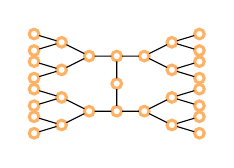
\begin{tikzpicture}[every node/.style={circle, draw, inner sep=2pt, minimum size=6mm}, scale = 0.35, transform shape]
    \tikzstyle{vertex}=[circle, draw = orange!60!white,fill=White,minimum size=10pt,inner sep=0pt, line width = 1.1pt]
    
    \foreach \label/\x/\y in  {1/3/3.5, 2/3/4.5, 3/3/2.5, 4/2/4.5, 5/4/4.5, 6/2/2.5, 7/4/2.5, 8/1/5, 9/1/4, 10/5/5, 11/5/4, 12/1/3, 13/1/2, 14/5/3, 15/5/2, 16/0/5.3, 17/0/4.7, 18/0/4.3, 19/0/3.7, 20/6/5.3, 21/6/4.7, 22/6/4.3, 23/6/3.7, 24/0/3.3, 25/0/2.7, 26/0/2.3, 27/0/1.7, 28/6/3.3, 29/6/2.7, 30/6/2.3, 31/6/1.7}
    \node[vertex] (G-\label) at (\x,\y){\makebox[0.35cm][c]{}};
    
    \foreach \from/\to in {1/2, 1/3, 2/4, 2/5, 3/6, 3/7, 4/8, 4/9, 5/10, 5/11, 6/12, 6/13, 7/14, 7/15, 8/16, 8/17, 9/18, 9/19, 10/20, 10/21, 11/22, 11/23, 12/24, 12/25, 13/26, 13/27, 14/28, 14/29, 15/30, 15/31}
    \draw (G-\from) -- (G-\to) ;
\end{tikzpicture} &

% Structure D - Chain
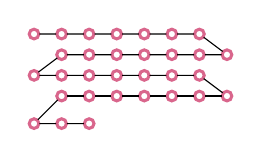
\begin{tikzpicture}[every node/.style={circle, draw, inner sep=2pt, minimum size=6mm}, scale = 0.35, transform shape]
    \tikzstyle{vertex}=[circle, draw = purple!60!white,fill=White,minimum size=10pt,inner sep=0pt, line width = 1.1 pt]
    
    \foreach \label/\x/\y in {30/1/2.25, 28/2/2.25, 26/3/2.25, 24/4/2.25, 22/5/2.25, 20/6/2.25, 18/7/2.25, 16/8/1.5, 
                     14/7/1.5, 12/6/1.5, 10/5/1.5, 8/4/1.5, 6/3/1.5, 4/2/1.5, 2/1/0.75, 1/2/0.75, 
                     3/3/0.75, 5/4/0.75, 7/5/0.75, 9/6/0.75, 11/7/0.75, 13/8/0, 15/7/0, 17/6/0, 
                     19/5/0, 21/4/0, 23/3/0, 25/2/0, 27/1/-1, 29/2/-1, 31/3/-1}
    \node[vertex] (G-\label) at (\x,\y) {\makebox[0.35cm][c]{}};

    
    \foreach \from/\to in {1/3, 3/5, 5/7, 7/9, 9/11, 11/13, 13/15, 15/17, 17/19, 19/21, 21/23, 23/25, 25/27, 27/29, 29/31, 1/2, 2/4, 4/6, 6/8, 8/10, 10/12, 12/14, 14/16, 16/18, 18/20, 20/22, 22/24, 24/26, 26/28, 28/30}
    \draw (G-\from) -- (G-\to) ;
\end{tikzpicture} \\
{Structure A} & {Structure B} & {Structure C} & {Structure D} \\
Star & 5-nary tree & Binary tree & Chain \\
\end{tabular}}
\begin{center}
\begin{tabular}{cccc}
% Structure A - Star

\begin{tikzpicture}[every node/.style={circle, draw, inner sep=2pt, minimum size=6mm}, scale = 0.35, transform shape]
    \tikzstyle{vertex}=[circle, draw = blue!60!white,fill=White,minimum size=10pt,inner sep=0pt, line width = 1.1pt]
    
    \foreach \label in {2,3,4,5,6,7,8,9}
    {
    \draw  (0,0) -- ({(\label-2)*12}:2cm);
    \node[vertex] (\label) at ({(\label-2)*12}:2cm) {\makebox[0.35cm][c]{\makebox[0.35cm][c]{}}};
    }
    \foreach \label in {10,11,12,13,14,15,16,17,18,19,20,21,22,23,24,25,26,27,28,29,30,31}
    {
    \draw  (0,0) -- ({(\label-2)*12}:2cm);
    \node[vertex] (\label) at ({(\label-2)*12}:2cm) {\makebox[0.35cm][c]{}};
    }
    \node[vertex] (base) at (0,0) {};
\end{tikzpicture} &

% Structure B - 5-nary tree
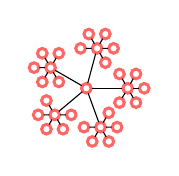
\begin{tikzpicture}[every node/.style={circle, draw, inner sep=2pt, minimum size=6mm}, scale = 0.35, transform shape]
    \tikzstyle{vertex}=[circle, draw = red!60!white,fill=White,minimum size=10pt,inner sep=0pt, line width = 1.1pt]
    
    \node[vertex] (base) at (0,0) {};
    
    \foreach \labelngle/\label in {75/2, 360/8, 290/14, 220/20, 150/26}{
        \node[vertex] (noeud\label) at (\labelngle:1.5cm) {\makebox[0.35cm][c]{}};
        \draw (base) -- (noeud\label);
    }
    
    \foreach \labelngle/\label in {360/4, 60/5, 120/6, 180/7, 300/3}{
        \node[vertex] (noeud\label) at ([shift={(\labelngle:0.6cm)}]noeud2) {\makebox[0.35cm][c]{}};
        \draw (noeud2) -- (noeud\label);
    }
    
    \foreach \labelngle/\label in {360/10, 60/11, 120/12, 240/13, 300/9}{
        \node[vertex] (noeud\label) at ([shift={(\labelngle:0.6cm)}]noeud8) {\makebox[0.35cm][c]{}};
        \draw (noeud8) -- (noeud\label);
    }
    
    \foreach \labelngle/\label in {60/15, 360/16, 300/17, 240/18, 180/19}{
        \node[vertex] (noeud\label) at ([shift={(\labelngle:0.6cm)}]noeud14) {\makebox[0.35cm][c]{}};
        \draw (noeud14) -- (noeud\label);
    }
    
    \foreach \labelngle/\label in {360/21, 300/22, 240/23, 180/24, 120/25}{
        \node[vertex] (noeud\label) at ([shift={(\labelngle:0.6cm)}]noeud20) {\makebox[0.35cm][c]{}};
        \draw (noeud20) -- (noeud\label);
    }
    
    \foreach \labelngle/\label in {180/29, 60/31, 120/30, 240/28, 300/27}{
        \node[vertex] (noeud\label) at ([shift={(\labelngle:0.6cm)}]noeud26) {\makebox[0.35cm][c]{}};
        \draw (noeud26) -- (noeud\label);
    }
\end{tikzpicture} &

% Structure C - Binary tree
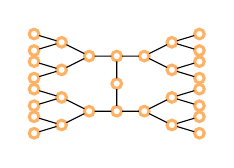
\begin{tikzpicture}[every node/.style={circle, draw, inner sep=2pt, minimum size=6mm}, scale = 0.35, transform shape]
    \tikzstyle{vertex}=[circle, draw = orange!60!white,fill=White,minimum size=10pt,inner sep=0pt, line width = 1.1pt]
    
    \foreach \label/\x/\y in  {1/3/3.5, 2/3/4.5, 3/3/2.5, 4/2/4.5, 5/4/4.5, 6/2/2.5, 7/4/2.5, 8/1/5, 9/1/4, 10/5/5, 11/5/4, 12/1/3, 13/1/2, 14/5/3, 15/5/2, 16/0/5.3, 17/0/4.7, 18/0/4.3, 19/0/3.7, 20/6/5.3, 21/6/4.7, 22/6/4.3, 23/6/3.7, 24/0/3.3, 25/0/2.7, 26/0/2.3, 27/0/1.7, 28/6/3.3, 29/6/2.7, 30/6/2.3, 31/6/1.7}
    \node[vertex] (G-\label) at (\x,\y){\makebox[0.35cm][c]{}};
    
    \foreach \from/\to in {1/2, 1/3, 2/4, 2/5, 3/6, 3/7, 4/8, 4/9, 5/10, 5/11, 6/12, 6/13, 7/14, 7/15, 8/16, 8/17, 9/18, 9/19, 10/20, 10/21, 11/22, 11/23, 12/24, 12/25, 13/26, 13/27, 14/28, 14/29, 15/30, 15/31}
    \draw (G-\from) -- (G-\to) ;
\end{tikzpicture} &

% Structure D - Chain
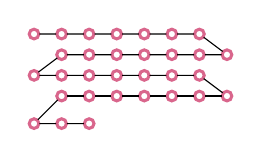
\begin{tikzpicture}[every node/.style={circle, draw, inner sep=2pt, minimum size=6mm}, scale = 0.35, transform shape]
    \tikzstyle{vertex}=[circle, draw = purple!60!white,fill=White,minimum size=10pt,inner sep=0pt, line width = 1.1 pt]
    
    \foreach \label/\x/\y in {30/1/2.25, 28/2/2.25, 26/3/2.25, 24/4/2.25, 22/5/2.25, 20/6/2.25, 18/7/2.25, 16/8/1.5, 
                     14/7/1.5, 12/6/1.5, 10/5/1.5, 8/4/1.5, 6/3/1.5, 4/2/1.5, 2/1/0.75, 1/2/0.75, 
                     3/3/0.75, 5/4/0.75, 7/5/0.75, 9/6/0.75, 11/7/0.75, 13/8/0, 15/7/0, 17/6/0, 
                     19/5/0, 21/4/0, 23/3/0, 25/2/0, 27/1/-1, 29/2/-1, 31/3/-1}
    \node[vertex] (G-\label) at (\x,\y) {\makebox[0.35cm][c]{}};

    
    \foreach \from/\to in {1/3, 3/5, 5/7, 7/9, 9/11, 11/13, 13/15, 15/17, 17/19, 19/21, 21/23, 23/25, 25/27, 27/29, 29/31, 1/2, 2/4, 4/6, 6/8, 8/10, 10/12, 12/14, 14/16, 16/18, 18/20, 20/22, 22/24, 24/26, 26/28, 28/30}
    \draw (G-\from) -- (G-\to) ;
\end{tikzpicture} \\
{Structure A} & {Structure B} & {Structure C} & {Structure D} \\
Star & 5-nary tree & Binary tree & Chain \\
\end{tabular}
\end{center}
\textbf{Question:} How does tree structure affect the distribution of $S_{31} = \sum_{v=1}^{31} X_v$?
\end{frame}

\begin{frame}{Numerical Illustration: Tree Structures}
\begin{center}
\vfill
\resizebox{!}{0.4\textwidth}{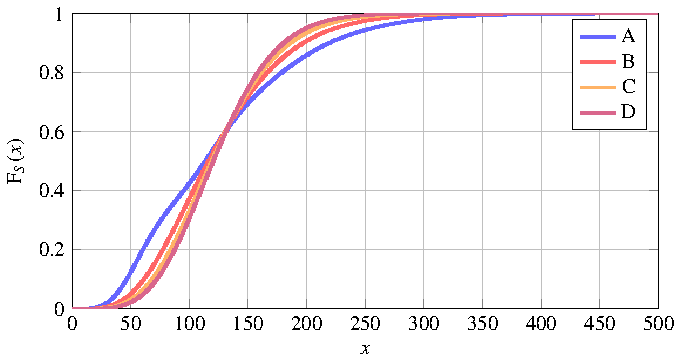
\includegraphics{Figures/structures_cdf.pdf}}
% \end{center}
\vfill
% \resizebox{!}{0.8\textwidth}
% {\begin{tabular}{cccc}
% Structure A - Star

\begin{tikzpicture}[every node/.style={circle, draw, inner sep=2pt, minimum size=6mm}, scale = 0.35, transform shape]
    \tikzstyle{vertex}=[circle, draw = blue!60!white,fill=White,minimum size=10pt,inner sep=0pt, line width = 1.1pt]
    
    \foreach \label in {2,3,4,5,6,7,8,9}
    {
    \draw  (0,0) -- ({(\label-2)*12}:2cm);
    \node[vertex] (\label) at ({(\label-2)*12}:2cm) {\makebox[0.35cm][c]{\makebox[0.35cm][c]{}}};
    }
    \foreach \label in {10,11,12,13,14,15,16,17,18,19,20,21,22,23,24,25,26,27,28,29,30,31}
    {
    \draw  (0,0) -- ({(\label-2)*12}:2cm);
    \node[vertex] (\label) at ({(\label-2)*12}:2cm) {\makebox[0.35cm][c]{}};
    }
    \node[vertex] (base) at (0,0) {};
\end{tikzpicture} &

% Structure B - 5-nary tree
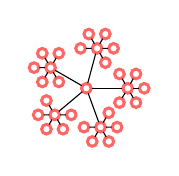
\begin{tikzpicture}[every node/.style={circle, draw, inner sep=2pt, minimum size=6mm}, scale = 0.35, transform shape]
    \tikzstyle{vertex}=[circle, draw = red!60!white,fill=White,minimum size=10pt,inner sep=0pt, line width = 1.1pt]
    
    \node[vertex] (base) at (0,0) {};
    
    \foreach \labelngle/\label in {75/2, 360/8, 290/14, 220/20, 150/26}{
        \node[vertex] (noeud\label) at (\labelngle:1.5cm) {\makebox[0.35cm][c]{}};
        \draw (base) -- (noeud\label);
    }
    
    \foreach \labelngle/\label in {360/4, 60/5, 120/6, 180/7, 300/3}{
        \node[vertex] (noeud\label) at ([shift={(\labelngle:0.6cm)}]noeud2) {\makebox[0.35cm][c]{}};
        \draw (noeud2) -- (noeud\label);
    }
    
    \foreach \labelngle/\label in {360/10, 60/11, 120/12, 240/13, 300/9}{
        \node[vertex] (noeud\label) at ([shift={(\labelngle:0.6cm)}]noeud8) {\makebox[0.35cm][c]{}};
        \draw (noeud8) -- (noeud\label);
    }
    
    \foreach \labelngle/\label in {60/15, 360/16, 300/17, 240/18, 180/19}{
        \node[vertex] (noeud\label) at ([shift={(\labelngle:0.6cm)}]noeud14) {\makebox[0.35cm][c]{}};
        \draw (noeud14) -- (noeud\label);
    }
    
    \foreach \labelngle/\label in {360/21, 300/22, 240/23, 180/24, 120/25}{
        \node[vertex] (noeud\label) at ([shift={(\labelngle:0.6cm)}]noeud20) {\makebox[0.35cm][c]{}};
        \draw (noeud20) -- (noeud\label);
    }
    
    \foreach \labelngle/\label in {180/29, 60/31, 120/30, 240/28, 300/27}{
        \node[vertex] (noeud\label) at ([shift={(\labelngle:0.6cm)}]noeud26) {\makebox[0.35cm][c]{}};
        \draw (noeud26) -- (noeud\label);
    }
\end{tikzpicture} &

% Structure C - Binary tree
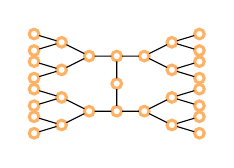
\begin{tikzpicture}[every node/.style={circle, draw, inner sep=2pt, minimum size=6mm}, scale = 0.35, transform shape]
    \tikzstyle{vertex}=[circle, draw = orange!60!white,fill=White,minimum size=10pt,inner sep=0pt, line width = 1.1pt]
    
    \foreach \label/\x/\y in  {1/3/3.5, 2/3/4.5, 3/3/2.5, 4/2/4.5, 5/4/4.5, 6/2/2.5, 7/4/2.5, 8/1/5, 9/1/4, 10/5/5, 11/5/4, 12/1/3, 13/1/2, 14/5/3, 15/5/2, 16/0/5.3, 17/0/4.7, 18/0/4.3, 19/0/3.7, 20/6/5.3, 21/6/4.7, 22/6/4.3, 23/6/3.7, 24/0/3.3, 25/0/2.7, 26/0/2.3, 27/0/1.7, 28/6/3.3, 29/6/2.7, 30/6/2.3, 31/6/1.7}
    \node[vertex] (G-\label) at (\x,\y){\makebox[0.35cm][c]{}};
    
    \foreach \from/\to in {1/2, 1/3, 2/4, 2/5, 3/6, 3/7, 4/8, 4/9, 5/10, 5/11, 6/12, 6/13, 7/14, 7/15, 8/16, 8/17, 9/18, 9/19, 10/20, 10/21, 11/22, 11/23, 12/24, 12/25, 13/26, 13/27, 14/28, 14/29, 15/30, 15/31}
    \draw (G-\from) -- (G-\to) ;
\end{tikzpicture} &

% Structure D - Chain
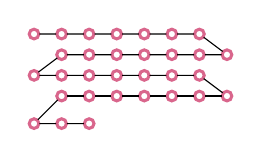
\begin{tikzpicture}[every node/.style={circle, draw, inner sep=2pt, minimum size=6mm}, scale = 0.35, transform shape]
    \tikzstyle{vertex}=[circle, draw = purple!60!white,fill=White,minimum size=10pt,inner sep=0pt, line width = 1.1 pt]
    
    \foreach \label/\x/\y in {30/1/2.25, 28/2/2.25, 26/3/2.25, 24/4/2.25, 22/5/2.25, 20/6/2.25, 18/7/2.25, 16/8/1.5, 
                     14/7/1.5, 12/6/1.5, 10/5/1.5, 8/4/1.5, 6/3/1.5, 4/2/1.5, 2/1/0.75, 1/2/0.75, 
                     3/3/0.75, 5/4/0.75, 7/5/0.75, 9/6/0.75, 11/7/0.75, 13/8/0, 15/7/0, 17/6/0, 
                     19/5/0, 21/4/0, 23/3/0, 25/2/0, 27/1/-1, 29/2/-1, 31/3/-1}
    \node[vertex] (G-\label) at (\x,\y) {\makebox[0.35cm][c]{}};

    
    \foreach \from/\to in {1/3, 3/5, 5/7, 7/9, 9/11, 11/13, 13/15, 15/17, 17/19, 19/21, 21/23, 23/25, 25/27, 27/29, 29/31, 1/2, 2/4, 4/6, 6/8, 8/10, 10/12, 12/14, 14/16, 16/18, 18/20, 20/22, 22/24, 24/26, 26/28, 28/30}
    \draw (G-\from) -- (G-\to) ;
\end{tikzpicture} \\
{Structure A} & {Structure B} & {Structure C} & {Structure D} \\
Star & 5-nary tree & Binary tree & Chain \\
\end{tabular}}
% \begin{center}
\begin{tabular}{cccc}
% Structure A - Star

\begin{tikzpicture}[every node/.style={circle, draw, inner sep=2pt, minimum size=6mm}, scale = 0.35, transform shape]
    \tikzstyle{vertex}=[circle, draw = blue!60!white,fill=White,minimum size=10pt,inner sep=0pt, line width = 1.1pt]
    
    \foreach \label in {2,3,4,5,6,7,8,9}
    {
    \draw  (0,0) -- ({(\label-2)*12}:2cm);
    \node[vertex] (\label) at ({(\label-2)*12}:2cm) {\makebox[0.35cm][c]{\makebox[0.35cm][c]{}}};
    }
    \foreach \label in {10,11,12,13,14,15,16,17,18,19,20,21,22,23,24,25,26,27,28,29,30,31}
    {
    \draw  (0,0) -- ({(\label-2)*12}:2cm);
    \node[vertex] (\label) at ({(\label-2)*12}:2cm) {\makebox[0.35cm][c]{}};
    }
    \node[vertex] (base) at (0,0) {};
\end{tikzpicture} &

% Structure B - 5-nary tree
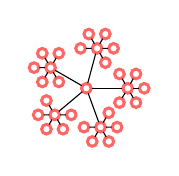
\begin{tikzpicture}[every node/.style={circle, draw, inner sep=2pt, minimum size=6mm}, scale = 0.35, transform shape]
    \tikzstyle{vertex}=[circle, draw = red!60!white,fill=White,minimum size=10pt,inner sep=0pt, line width = 1.1pt]
    
    \node[vertex] (base) at (0,0) {};
    
    \foreach \labelngle/\label in {75/2, 360/8, 290/14, 220/20, 150/26}{
        \node[vertex] (noeud\label) at (\labelngle:1.5cm) {\makebox[0.35cm][c]{}};
        \draw (base) -- (noeud\label);
    }
    
    \foreach \labelngle/\label in {360/4, 60/5, 120/6, 180/7, 300/3}{
        \node[vertex] (noeud\label) at ([shift={(\labelngle:0.6cm)}]noeud2) {\makebox[0.35cm][c]{}};
        \draw (noeud2) -- (noeud\label);
    }
    
    \foreach \labelngle/\label in {360/10, 60/11, 120/12, 240/13, 300/9}{
        \node[vertex] (noeud\label) at ([shift={(\labelngle:0.6cm)}]noeud8) {\makebox[0.35cm][c]{}};
        \draw (noeud8) -- (noeud\label);
    }
    
    \foreach \labelngle/\label in {60/15, 360/16, 300/17, 240/18, 180/19}{
        \node[vertex] (noeud\label) at ([shift={(\labelngle:0.6cm)}]noeud14) {\makebox[0.35cm][c]{}};
        \draw (noeud14) -- (noeud\label);
    }
    
    \foreach \labelngle/\label in {360/21, 300/22, 240/23, 180/24, 120/25}{
        \node[vertex] (noeud\label) at ([shift={(\labelngle:0.6cm)}]noeud20) {\makebox[0.35cm][c]{}};
        \draw (noeud20) -- (noeud\label);
    }
    
    \foreach \labelngle/\label in {180/29, 60/31, 120/30, 240/28, 300/27}{
        \node[vertex] (noeud\label) at ([shift={(\labelngle:0.6cm)}]noeud26) {\makebox[0.35cm][c]{}};
        \draw (noeud26) -- (noeud\label);
    }
\end{tikzpicture} &

% Structure C - Binary tree
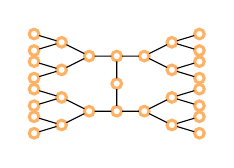
\begin{tikzpicture}[every node/.style={circle, draw, inner sep=2pt, minimum size=6mm}, scale = 0.35, transform shape]
    \tikzstyle{vertex}=[circle, draw = orange!60!white,fill=White,minimum size=10pt,inner sep=0pt, line width = 1.1pt]
    
    \foreach \label/\x/\y in  {1/3/3.5, 2/3/4.5, 3/3/2.5, 4/2/4.5, 5/4/4.5, 6/2/2.5, 7/4/2.5, 8/1/5, 9/1/4, 10/5/5, 11/5/4, 12/1/3, 13/1/2, 14/5/3, 15/5/2, 16/0/5.3, 17/0/4.7, 18/0/4.3, 19/0/3.7, 20/6/5.3, 21/6/4.7, 22/6/4.3, 23/6/3.7, 24/0/3.3, 25/0/2.7, 26/0/2.3, 27/0/1.7, 28/6/3.3, 29/6/2.7, 30/6/2.3, 31/6/1.7}
    \node[vertex] (G-\label) at (\x,\y){\makebox[0.35cm][c]{}};
    
    \foreach \from/\to in {1/2, 1/3, 2/4, 2/5, 3/6, 3/7, 4/8, 4/9, 5/10, 5/11, 6/12, 6/13, 7/14, 7/15, 8/16, 8/17, 9/18, 9/19, 10/20, 10/21, 11/22, 11/23, 12/24, 12/25, 13/26, 13/27, 14/28, 14/29, 15/30, 15/31}
    \draw (G-\from) -- (G-\to) ;
\end{tikzpicture} &

% Structure D - Chain
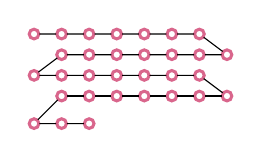
\begin{tikzpicture}[every node/.style={circle, draw, inner sep=2pt, minimum size=6mm}, scale = 0.35, transform shape]
    \tikzstyle{vertex}=[circle, draw = purple!60!white,fill=White,minimum size=10pt,inner sep=0pt, line width = 1.1 pt]
    
    \foreach \label/\x/\y in {30/1/2.25, 28/2/2.25, 26/3/2.25, 24/4/2.25, 22/5/2.25, 20/6/2.25, 18/7/2.25, 16/8/1.5, 
                     14/7/1.5, 12/6/1.5, 10/5/1.5, 8/4/1.5, 6/3/1.5, 4/2/1.5, 2/1/0.75, 1/2/0.75, 
                     3/3/0.75, 5/4/0.75, 7/5/0.75, 9/6/0.75, 11/7/0.75, 13/8/0, 15/7/0, 17/6/0, 
                     19/5/0, 21/4/0, 23/3/0, 25/2/0, 27/1/-1, 29/2/-1, 31/3/-1}
    \node[vertex] (G-\label) at (\x,\y) {\makebox[0.35cm][c]{}};

    
    \foreach \from/\to in {1/3, 3/5, 5/7, 7/9, 9/11, 11/13, 13/15, 15/17, 17/19, 19/21, 21/23, 23/25, 25/27, 27/29, 29/31, 1/2, 2/4, 4/6, 6/8, 8/10, 10/12, 12/14, 14/16, 16/18, 18/20, 20/22, 22/24, 24/26, 26/28, 28/30}
    \draw (G-\from) -- (G-\to) ;
\end{tikzpicture} \\
{Structure A} & {Structure B} & {Structure C} & {Structure D} \\
% Star & 5-nary tree & Binary tree & Chain \\
\end{tabular}
\end{center}
\end{frame}

\begin{frame}{Numerical Illustration: Risk allocation of TVaR}
\begin{itemize}
    \item At confidence level $\kappa$: $\text{TVaR}_{\kappa}(X) = \mathbb{E}[X \mid X > \text{VaR}_{\kappa}(X)]$    
    \item Our construction allows for \al{efficient exact computation} of:
    \begin{itemize}
        % \item TVaR of the aggregate loss $S$
        % \item Individual risk contributions to TVaR: $\text{TVaR}_{\kappa}(X_v \mid S)$
        \item Allocation of total risk to each component
    \end{itemize}
\end{itemize}
\begin{center}
% \vfill
\resizebox{!}{0.3\textwidth}{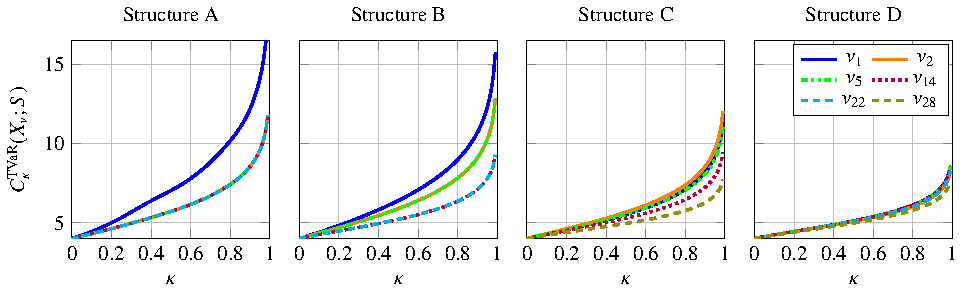
\includegraphics{Figures/contributions.pdf}}
% \end{center}
\vspace{-0.5cm}
% \resizebox{!}{0.8\textwidth}
% {\begin{tabular}{cccc}
% Structure A - Star

\begin{tikzpicture}[every node/.style={circle, draw, inner sep=2pt, minimum size=6mm}, scale = 0.35, transform shape]
    \tikzstyle{vertex}=[circle, draw = blue!60!white,fill=White,minimum size=10pt,inner sep=0pt, line width = 1.1pt]
    
    \foreach \label in {2,3,4,5,6,7,8,9}
    {
    \draw  (0,0) -- ({(\label-2)*12}:2cm);
    \node[vertex] (\label) at ({(\label-2)*12}:2cm) {\makebox[0.35cm][c]{\makebox[0.35cm][c]{}}};
    }
    \foreach \label in {10,11,12,13,14,15,16,17,18,19,20,21,22,23,24,25,26,27,28,29,30,31}
    {
    \draw  (0,0) -- ({(\label-2)*12}:2cm);
    \node[vertex] (\label) at ({(\label-2)*12}:2cm) {\makebox[0.35cm][c]{}};
    }
    \node[vertex] (base) at (0,0) {};
\end{tikzpicture} &

% Structure B - 5-nary tree
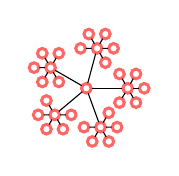
\begin{tikzpicture}[every node/.style={circle, draw, inner sep=2pt, minimum size=6mm}, scale = 0.35, transform shape]
    \tikzstyle{vertex}=[circle, draw = red!60!white,fill=White,minimum size=10pt,inner sep=0pt, line width = 1.1pt]
    
    \node[vertex] (base) at (0,0) {};
    
    \foreach \labelngle/\label in {75/2, 360/8, 290/14, 220/20, 150/26}{
        \node[vertex] (noeud\label) at (\labelngle:1.5cm) {\makebox[0.35cm][c]{}};
        \draw (base) -- (noeud\label);
    }
    
    \foreach \labelngle/\label in {360/4, 60/5, 120/6, 180/7, 300/3}{
        \node[vertex] (noeud\label) at ([shift={(\labelngle:0.6cm)}]noeud2) {\makebox[0.35cm][c]{}};
        \draw (noeud2) -- (noeud\label);
    }
    
    \foreach \labelngle/\label in {360/10, 60/11, 120/12, 240/13, 300/9}{
        \node[vertex] (noeud\label) at ([shift={(\labelngle:0.6cm)}]noeud8) {\makebox[0.35cm][c]{}};
        \draw (noeud8) -- (noeud\label);
    }
    
    \foreach \labelngle/\label in {60/15, 360/16, 300/17, 240/18, 180/19}{
        \node[vertex] (noeud\label) at ([shift={(\labelngle:0.6cm)}]noeud14) {\makebox[0.35cm][c]{}};
        \draw (noeud14) -- (noeud\label);
    }
    
    \foreach \labelngle/\label in {360/21, 300/22, 240/23, 180/24, 120/25}{
        \node[vertex] (noeud\label) at ([shift={(\labelngle:0.6cm)}]noeud20) {\makebox[0.35cm][c]{}};
        \draw (noeud20) -- (noeud\label);
    }
    
    \foreach \labelngle/\label in {180/29, 60/31, 120/30, 240/28, 300/27}{
        \node[vertex] (noeud\label) at ([shift={(\labelngle:0.6cm)}]noeud26) {\makebox[0.35cm][c]{}};
        \draw (noeud26) -- (noeud\label);
    }
\end{tikzpicture} &

% Structure C - Binary tree
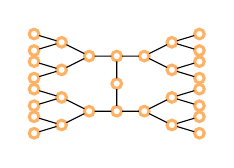
\begin{tikzpicture}[every node/.style={circle, draw, inner sep=2pt, minimum size=6mm}, scale = 0.35, transform shape]
    \tikzstyle{vertex}=[circle, draw = orange!60!white,fill=White,minimum size=10pt,inner sep=0pt, line width = 1.1pt]
    
    \foreach \label/\x/\y in  {1/3/3.5, 2/3/4.5, 3/3/2.5, 4/2/4.5, 5/4/4.5, 6/2/2.5, 7/4/2.5, 8/1/5, 9/1/4, 10/5/5, 11/5/4, 12/1/3, 13/1/2, 14/5/3, 15/5/2, 16/0/5.3, 17/0/4.7, 18/0/4.3, 19/0/3.7, 20/6/5.3, 21/6/4.7, 22/6/4.3, 23/6/3.7, 24/0/3.3, 25/0/2.7, 26/0/2.3, 27/0/1.7, 28/6/3.3, 29/6/2.7, 30/6/2.3, 31/6/1.7}
    \node[vertex] (G-\label) at (\x,\y){\makebox[0.35cm][c]{}};
    
    \foreach \from/\to in {1/2, 1/3, 2/4, 2/5, 3/6, 3/7, 4/8, 4/9, 5/10, 5/11, 6/12, 6/13, 7/14, 7/15, 8/16, 8/17, 9/18, 9/19, 10/20, 10/21, 11/22, 11/23, 12/24, 12/25, 13/26, 13/27, 14/28, 14/29, 15/30, 15/31}
    \draw (G-\from) -- (G-\to) ;
\end{tikzpicture} &

% Structure D - Chain
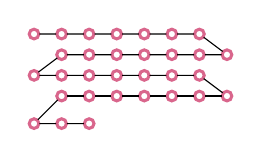
\begin{tikzpicture}[every node/.style={circle, draw, inner sep=2pt, minimum size=6mm}, scale = 0.35, transform shape]
    \tikzstyle{vertex}=[circle, draw = purple!60!white,fill=White,minimum size=10pt,inner sep=0pt, line width = 1.1 pt]
    
    \foreach \label/\x/\y in {30/1/2.25, 28/2/2.25, 26/3/2.25, 24/4/2.25, 22/5/2.25, 20/6/2.25, 18/7/2.25, 16/8/1.5, 
                     14/7/1.5, 12/6/1.5, 10/5/1.5, 8/4/1.5, 6/3/1.5, 4/2/1.5, 2/1/0.75, 1/2/0.75, 
                     3/3/0.75, 5/4/0.75, 7/5/0.75, 9/6/0.75, 11/7/0.75, 13/8/0, 15/7/0, 17/6/0, 
                     19/5/0, 21/4/0, 23/3/0, 25/2/0, 27/1/-1, 29/2/-1, 31/3/-1}
    \node[vertex] (G-\label) at (\x,\y) {\makebox[0.35cm][c]{}};

    
    \foreach \from/\to in {1/3, 3/5, 5/7, 7/9, 9/11, 11/13, 13/15, 15/17, 17/19, 19/21, 21/23, 23/25, 25/27, 27/29, 29/31, 1/2, 2/4, 4/6, 6/8, 8/10, 10/12, 12/14, 14/16, 16/18, 18/20, 20/22, 22/24, 24/26, 26/28, 28/30}
    \draw (G-\from) -- (G-\to) ;
\end{tikzpicture} \\
{Structure A} & {Structure B} & {Structure C} & {Structure D} \\
Star & 5-nary tree & Binary tree & Chain \\
\end{tabular}}
% \begin{center}
\begin{tabular}{cccc}
% Structure A - Star
\hspace{0.8cm} 

\begin{tikzpicture}[every node/.style={circle, draw, inner sep=2pt, minimum size=6mm}, scale = 0.35, transform shape]
    \tikzstyle{vertex}=[circle, draw = black,fill=White,minimum size=10pt,inner sep=0pt, line width = 1.1pt]
    
    \foreach \label in {2,3,4,5,6,7,8,9}
    {
    \draw  (0,0) -- ({(\label-2)*12}:2cm);
    \node[vertex] (\label) at ({(\label-2)*12}:2cm) {\makebox[0.35cm][c]{\makebox[0.35cm][c]{}}};
    }
    \foreach \label in {10,11,12,13,14,15,16,17,18,19,20,21,22,23,24,25,26,27,28,29,30,31}
    {
    \draw  (0,0) -- ({(\label-2)*12}:2cm);
    \node[vertex] (\label) at ({(\label-2)*12}:2cm) {\makebox[0.35cm][c]{}};
    }
    \node[vertex, fill = blue, draw = blue] (base) at (0,0) {};
    \node[vertex, fill = orange, draw = orange] (base) at (2) {};
    \node[vertex, fill = green, draw = green] (base) at (5) {};
    \node[vertex, fill = purple, draw = purple] (base) at (14) {};
    \node[vertex, fill = cyan, draw = cyan] (base) at (22) {};
    \node[vertex, fill = olive, draw = olive] (base) at (28) {};
    
\end{tikzpicture} &
\hspace{0.6cm}
% Structure B - 5-nary tree
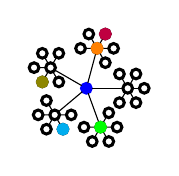
\begin{tikzpicture}[every node/.style={circle, draw, inner sep=2pt, minimum size=6mm}, scale = 0.35, transform shape]
    \tikzstyle{vertex}=[circle, draw = black,fill=White,minimum size=10pt,inner sep=0pt, line width = 1.1pt]
    
    \node[vertex, draw = blue, fill = blue] (base) at (0,0) {};
    
    \foreach \labelngle/\label in {75/2, 360/8, 290/14, 220/20, 150/26}{
        \node[vertex] (noeud\label) at (\labelngle:1.5cm) {\makebox[0.35cm][c]{}};
        \draw (base) -- (noeud\label);
    }
    
    \foreach \labelngle/\label in {360/4, 60/5, 120/6, 180/7, 300/3}{
        \node[vertex] (noeud\label) at ([shift={(\labelngle:0.6cm)}]noeud2) {\makebox[0.35cm][c]{}};
        \draw (noeud2) -- (noeud\label);
    }
    
    \foreach \labelngle/\label in {360/10, 60/11, 120/12, 240/13, 300/9}{
        \node[vertex] (noeud\label) at ([shift={(\labelngle:0.6cm)}]noeud8) {\makebox[0.35cm][c]{}};
        \draw (noeud8) -- (noeud\label);
    }
    
    \foreach \labelngle/\label in {60/15, 360/16, 300/17, 240/18, 180/19}{
        \node[vertex] (noeud\label) at ([shift={(\labelngle:0.6cm)}]noeud14) {\makebox[0.35cm][c]{}};
        \draw (noeud14) -- (noeud\label);
    }
    
    \foreach \labelngle/\label in {360/21, 300/22, 240/23, 180/24, 120/25}{
        \node[vertex] (noeud\label) at ([shift={(\labelngle:0.6cm)}]noeud20) {\makebox[0.35cm][c]{}};
        \draw (noeud20) -- (noeud\label);
    }
    
    \foreach \labelngle/\label in {180/29, 60/31, 120/30, 240/28, 300/27}{
        \node[vertex] (noeud\label) at ([shift={(\labelngle:0.6cm)}]noeud26) {\makebox[0.35cm][c]{}};
        \draw (noeud26) -- (noeud\label);
    }

    \node[vertex, fill = orange, draw = orange]  at (noeud2) {};
    \node[vertex, fill = purple, draw = purple]  at (noeud5) {};
    \node[vertex, fill = green, draw = green]  at (noeud14) {};
    \node[vertex, fill = cyan, draw = cyan]  at (noeud22) {};
    \node[vertex, fill = olive, draw = olive]  at (noeud28) {};
\end{tikzpicture} &
\hspace{0.2cm}
% Structure C - Binary tree
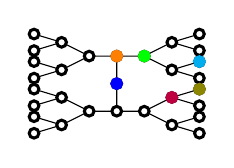
\begin{tikzpicture}[every node/.style={circle, draw, inner sep=2pt, minimum size=6mm}, scale = 0.35, transform shape]
    \tikzstyle{vertex}=[circle, draw = black,fill=White,minimum size=10pt,inner sep=0pt, line width = 1.1pt]
    
    \foreach \label/\x/\y in  {1/3/3.5, 2/3/4.5, 3/3/2.5, 4/2/4.5, 5/4/4.5, 6/2/2.5, 7/4/2.5, 8/1/5, 9/1/4, 10/5/5, 11/5/4, 12/1/3, 13/1/2, 14/5/3, 15/5/2, 16/0/5.3, 17/0/4.7, 18/0/4.3, 19/0/3.7, 20/6/5.3, 21/6/4.7, 22/6/4.3, 23/6/3.7, 24/0/3.3, 25/0/2.7, 26/0/2.3, 27/0/1.7, 28/6/3.3, 29/6/2.7, 30/6/2.3, 31/6/1.7}
    \node[vertex] (G-\label) at (\x,\y){\makebox[0.35cm][c]{}};
    
    \foreach \from/\to in {1/2, 1/3, 2/4, 2/5, 3/6, 3/7, 4/8, 4/9, 5/10, 5/11, 6/12, 6/13, 7/14, 7/15, 8/16, 8/17, 9/18, 9/19, 10/20, 10/21, 11/22, 11/23, 12/24, 12/25, 13/26, 13/27, 14/28, 14/29, 15/30, 15/31}
    \draw (G-\from) -- (G-\to) ;
    \node[vertex, fill = blue, draw = blue] at (G-1) {};
    \node[vertex, fill = orange, draw = orange] at (G-2) {};
    \node[vertex, fill = green, draw = green] at (G-5) {};
    \node[vertex, fill = purple, draw = purple] at (G-14) {};
    \node[vertex, fill = cyan, draw = cyan] at (G-22) {};
    \node[vertex, fill = olive, draw = olive] at (G-28) {};
\end{tikzpicture} &

% Structure D - Chain
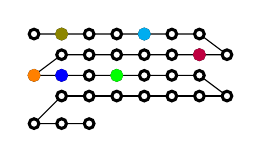
\begin{tikzpicture}[every node/.style={circle, draw, inner sep=2pt, minimum size=6mm}, scale = 0.35, transform shape]
    \tikzstyle{vertex}=[circle, draw = black,fill=White,minimum size=10pt,inner sep=0pt, line width = 1.1 pt]
    
    \foreach \label/\x/\y in {30/1/2.25, 28/2/2.25, 26/3/2.25, 24/4/2.25, 22/5/2.25, 20/6/2.25, 18/7/2.25, 16/8/1.5, 
                     14/7/1.5, 12/6/1.5, 10/5/1.5, 8/4/1.5, 6/3/1.5, 4/2/1.5, 2/1/0.75, 1/2/0.75, 
                     3/3/0.75, 5/4/0.75, 7/5/0.75, 9/6/0.75, 11/7/0.75, 13/8/0, 15/7/0, 17/6/0, 
                     19/5/0, 21/4/0, 23/3/0, 25/2/0, 27/1/-1, 29/2/-1, 31/3/-1}
    \node[vertex] (G-\label) at (\x,\y) {\makebox[0.35cm][c]{}};

    
    \foreach \from/\to in {1/3, 3/5, 5/7, 7/9, 9/11, 11/13, 13/15, 15/17, 17/19, 19/21, 21/23, 23/25, 25/27, 27/29, 29/31, 1/2, 2/4, 4/6, 6/8, 8/10, 10/12, 12/14, 14/16, 16/18, 18/20, 20/22, 22/24, 24/26, 26/28, 28/30}
    \draw (G-\from) -- (G-\to) ;
    \node[vertex, fill = blue, draw = blue] at (G-1) {};
    \node[vertex, fill = orange, draw = orange] at (G-2) {};
    \node[vertex, fill = green, draw = green] at (G-5) {};
    \node[vertex, fill = purple, draw = purple] at (G-14) {};
    \node[vertex, fill = cyan, draw = cyan] at (G-22) {};
    \node[vertex, fill = olive, draw = olive] at (G-28) {};
\end{tikzpicture} \\
\hspace{0.8cm} {Structure A} &
\hspace{0.6cm} {Structure B} & 
\hspace{0.2cm} {Structure C} & 
{Structure D} \\
% Star & 5-nary tree & Binary tree & Chain \\
\end{tabular}
\end{center}
\end{frame}

\begin{frame}{Asymptotic Behavior of Normalized Total Losses}
\begin{itemize}
    \item Same general settings
    \item $B_v \sim \text{NBinom}(r = 2, q = 1/3)$ such that $E[B_v] =4$ for all $v \in \mathcal{V}$.
\end{itemize}
\begin{center}
\begin{tabular}{cc}
\resizebox{!}{.45\textwidth}{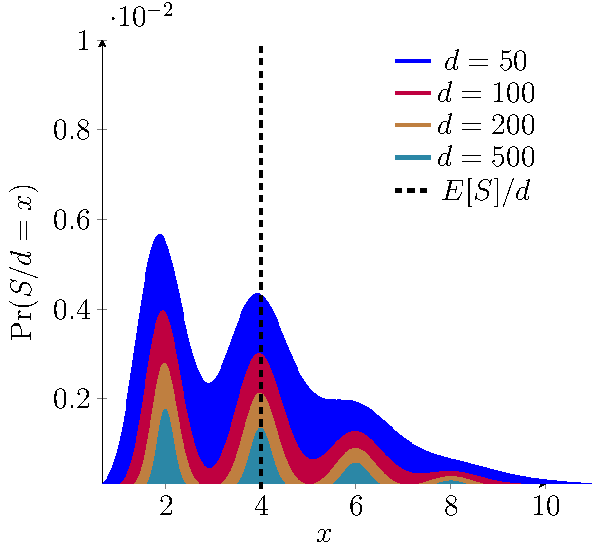
\includegraphics{Figures/star-fmp-sd.pdf}} &
\resizebox{!}{.45\textwidth}{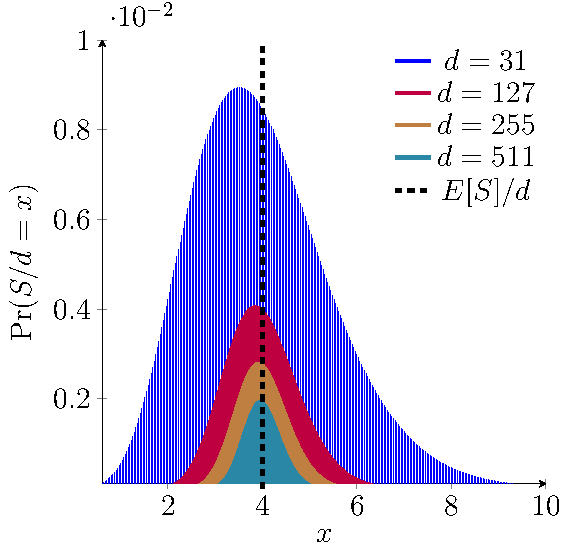
\includegraphics{Figures/binary-fmp-sd.pdf}} \\
{Pmf of $S_d^A/d$ (Star structure)} & 
{Pmf of $S_d^C/d$ (Binary structure)} \\
\end{tabular}
\end{center}
% \vspace{0.5cm}
% \begin{itemize}
%     \item As portfolio size $d$ increases, the normalized total loss $S_d/d$ converges in distribution
%     \item The limiting distribution depends on the tree structure
%     \item Star structure (A) shows higher variance in the limit compared to binary structure (B)
%     \item This confirms that centralized dependence structures lead to higher aggregate risk
% \end{itemize}
\end{frame}


% \begin{frame}{Risk Sharing: Definition and Optimal Rule}
%     \begin{itemize}
%         \item \al{Fair risk sharing rule:} a function $h: \boldsymbol{X} \mapsto (h_{v,n}(S_n))_{v \in [n]}$ that allocates the total cost $S_n = \sum_{v=1}^n X_v$ among $n$ participants such that:
%         \begin{equation*}
%         \sum_{v=1}^n h_{v,n}(S_n) = S_n
%         \quad \text{and} \quad
%         \mathbb{E}[h_{v,n}(S_n)] = \mathbb{E}[X_v] \quad \text{(fairness)}.
%         \end{equation*}
%         \pause
%         \item \al{Optimal rule:} the conditional expectation
%         \begin{equation*}
%         h_{i,n}^{\star}(S_n) = \mathbb{E}[X_i \mid S_n]
%         \end{equation*}
%         minimizes the mean squared error:
%         \begin{equation*}
%         \mathbb{E}\left[(X_i - h(S_n))^2\right],
%         \end{equation*}
%         over all measurable functions $h(S_n)$.
%     \end{itemize}
% \end{frame}

\begin{frame}{Conclusion and Key Takeaways}

\end{frame}
\appendix

\begin{frame}[allowframebreaks]{References}
\bibliography{references}
\bibliographystyle{apalike}
\end{frame}

\lastslide

\begin{frame}[label=backupSlide]
\frametitle{First backup slide}
\begin{itemize}
\item Lorem ipsum dolor sit amet, consectetur adipisicing elit, sed do eiusmod
tempor incididunt ut labore et dolore magna aliqua.
\item  Ut enim ad minim veniam, quis nostrud exercitation ullamco laboris nisi ut aliquip ex ea commodo consequat. 
\item Duis aute irure dolor in reprehenderit in voluptate velit esse
cillum dolore eu fugiat nulla pariatur. 
\end{itemize}
\hyperlink{firstSlide}{\beamergotobutton{Return to main slide}}
\end{frame}

\begin{frame}[label=anotherBackupSlide]
\frametitle{Another backup slide}
\begin{enumerate}
\item  Ut enim ad minim veniam, quis nostrud exercitation ullamco laboris nisi ut aliquip ex ea commodo consequat. 
\item Lorem ipsum dolor sit amet, consectetur adipisicing elit, sed do eiusmod
tempor incididunt ut labore et dolore magna aliqua.
\begin{enumerate}
\item Duis aute irure dolor in reprehenderit in voluptate velit esse
\item Cillum dolore eu fugiat nulla pariatur
\end{enumerate}
\item Lorem ipsum dolor sit amet, consectetur adipisicing elit, sed do eiusmod
tempor incididunt ut labore et dolore magna aliqua.
\end{enumerate}
\hyperlink{firstSlide}{\beamergotobutton{Return to main slide}}
\end{frame}

\end{document}